% Drawing 156-5/03-1 -- folder 156-5, batch 03, archive page 48 (PDF page 49).
% Transcription: croquis : deux ovales l'un au-dessus de l'autre, reliés par une flèche verticale $\varphi$ (surchargée d'un signe biffé). L'ovale du haut, surmonté d'une accolade marquée $I'$, contient trois points : un point isolé en haut à gauche, relié au point $b$ par un trait épais hachuré, et deux points $a \to b$ reliés par une flèche. L'ovale du bas, marqué $J'$ à gauche et souligné d'une accolade marquée $I$, contient deux points reliés par une flèche. À gauche de l'ovale du haut, un gribouillis biffé
% Kind: two ovals joined by phi, with points and arrows. Method 2 (schematic redraw from the facsimile). Status: ok.
% Notes: Upper oval under a brace I': an isolated point at the upper left joined to b by a thick hatched stroke, and a -> b. Lower oval, marked J' on the left, over a brace I: two points joined by an arrow. A vertical arrow phi joins them on the right. Omitted as struck: the sign scribbled out at the foot of the phi arrow, and the scribble at the left of the upper oval. Issue 128, 2026-11-09: struck material left out after a fresh check of the facsimile (struck-out material is not drawn). Redrawn 2026-11-09 (issue 128): to check again.
% Coordinates: 1 unit = 1 mm = 1/100 of the crop width (bbox in page fractions: [0.25, 0.2, 0.55, 0.36]).
% Redrawn by Claude (claude-opus-5-5), issue #73, 2026-11-07; not checked by a human; not compiled (no TeX in the session).
% Rights: reproduces part of the work -- behind RENDER_TRANSCRIPTS, never published by itself.
\documentclass[tikz,border=3pt]{standalone}
\usepackage{amsmath,amssymb}
\usetikzlibrary{patterns,arrows.meta}
\tikzset{pencil/.style={black!45}, struck/.style={black!35}, mark/.style={circle,draw,inner sep=1.3pt}, pt/.style={circle,fill,inner sep=0.9pt}, opt/.style={circle,draw,fill=white,inner sep=1.1pt}}
\begin{document}
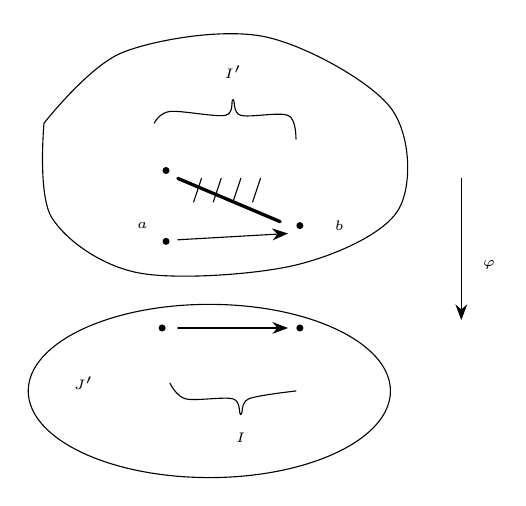
\begin{tikzpicture}[x=1mm,y=1mm,line cap=round,line join=round,font=\scriptsize]
\draw plot[smooth, tension=0.55] coordinates {(40,-22) (50,-13) (68,-11) (84,-20) (85,-33) (72,-40) (52,-41) (41,-34) (40,-22)};
\draw plot[smooth, tension=0.55] coordinates {(54,-22) (56,-20.5) (63,-21) (64,-19) (65,-21) (71,-21) (72,-24)};
\node[inner sep=1pt] at (64,-15.5) {\tiny $I'$};
\node[pt] at (55.5,-28) {};
\draw[very thick] (57,-29) -- (70,-34.5);
\draw (60,-29) -- (59,-32);
\draw (62.5,-29) -- (61.5,-32);
\draw (65,-29) -- (64,-32);
\draw (67.5,-29) -- (66.5,-32);
\node[pt] at (55.5,-37) {};
\node[inner sep=1pt] at (52.5,-35) {\tiny $a$};
\draw[-{Stealth[length=2mm]}] (57,-36.8) -- (71,-36);
\node[pt] at (72.5,-35) {};
\node[inner sep=1pt] at (77.5,-35) {\tiny $b$};
\draw (61,-56) ellipse[x radius=23, y radius=11];
\node[pt] at (55,-48) {};
\node[pt] at (72.5,-48) {};
\draw[-{Stealth[length=2mm]}] (57,-48) -- (71,-48);
\node[inner sep=1pt] at (45,-55) {\tiny $J'$};
\draw plot[smooth, tension=0.55] coordinates {(56,-55) (58,-57) (64,-57) (65,-59) (66,-57) (72,-56)};
\node[inner sep=1pt] at (65,-62) {\tiny $I$};
\draw[-{Stealth[length=2mm]}] (93,-29) -- (93,-47);
\node[inner sep=1pt] at (96.5,-40) {\tiny $\varphi$};
\end{tikzpicture}
\end{document}
